\documentclass[usepdftitle=false]{beamer}
\usepackage[utf8]{inputenc}
\usetheme{Singapore}
\usepackage{xcolor}
% \setbeamercovered{transparent}
%\usecolortheme{crane}
\title[IFT2505]{IFT 2505\\Programmation Linéaire\\Cycles et dégénérescence}
\author[Fabian Bastin]{Fabian Bastin\\DIRO\\Université de Montréal}
\date{}

\setbeamertemplate{footline}[frame number]

\usepackage{ulem}

\usepackage{tikz}
\newcommand*\circled[1]{\tikz[baseline=(char.base)]{
		\node[shape=circle,draw,inner sep=2pt] (char) {#1};}}

\def\ba{\boldsymbol{a}}
\def\bb{\boldsymbol{b}}
\def\bc{\boldsymbol{c}}
\def\be{\boldsymbol{e}}
\def\br{\boldsymbol{r}}
\def\bx{\boldsymbol{x}}
\def\by{\boldsymbol{y}}
\def\bz{\boldsymbol{z}}
\def\bA{\boldsymbol{A}}
\def\bB{\boldsymbol{B}}
\def\bD{\boldsymbol{D}}
\def\bzero{\boldsymbol{0}}

\begin{document}
\frame{\titlepage}

% 

\begin{frame}
\frametitle{Exemple: simplexe}

\[
\begin{matrix}
\ba_1 & \ba_2 & \ba_3 & \ba_4 & \ba_5 &\ba_6 &\ba_7 & \bb \\
\circled{$\frac{1}{4}$} & -60 & -\frac{1}{25} & 9 & 1 & 0 & 0 & 0 \\
\frac{1}{2} & -90 & -\frac{1}{50} & 3 & 0 & 1 & 0 & 0 \\
0 & 0 & 1 & 0 & 0 & 0 & 1 & 1 \\
-\frac{3}{4} & 150 & -\frac{1}{50} & 6 & 0 & 0 & 0 & 0
\end{matrix}
\]

\[
\begin{matrix}
\ba_1 & \ba_2 & \ba_3 & \ba_4 & \ba_5 &\ba_6 &\ba_7 & \bb \\
1 & -240 & -\frac{4}{25} & 36 & 4 & 0 & 0 & 0 \\
0 & 30 & \frac{3}{50} & -15 & -2 & 1 & 0 & 0 \\
0 & 0 & 1 & 0 & 0 & 0 & 1 & 1 \\
0 & -30 & -\frac{7}{50} & 33 & 3 & 0 & 0 & 0
\end{matrix}
\]

\end{frame}

\begin{frame}
\frametitle{Exemple}

\[
\begin{matrix}
\ba_1 & \ba_2 & \ba_3 & \ba_4 & \ba_5 &\ba_6 &\ba_7 & \bb \\
1 & -240 & -\frac{4}{25} & 36 & 4 & 0 & 0 & 0 \\
0 & \circled{30} & \frac{3}{50} & -15 & -2 & 1 & 0 & 0 \\
0 & 0 & 1 & 0 & 0 & 0 & 1 & 1 \\
0 & -30 & -\frac{7}{50} & 33 & 3 & 0 & 0 & 0
\end{matrix}
\]

\[
\begin{matrix}
\ba_1 & \ba_2 & \ba_3 & \ba_4 & \ba_5 &\ba_6 &\ba_7 & \bb \\
1 & 0 & \frac{8}{25} & -84 & -12 & 8 & 0 & 0 \\
0 & 1 & \frac{1}{500} & -\frac{1}{2} & -\frac{1}{15} & \frac{1}{30} & 0 & 0 \\
0 & 0 & 1 & 0 & 0 & 0 & 1 & 1 \\
0 & 0 & -\frac{2}{25} & 18 & 1 & 1 & 0 & 0
\end{matrix}
\]

\end{frame}

\begin{frame}
\frametitle{Exemple}

\[
\begin{matrix}
\ba_1 & \ba_2 & \ba_3 & \ba_4 & \ba_5 &\ba_6 &\ba_7 & \bb \\
1 & 0 & \frac{8}{25} & -84 & -12 & 8 & 0 & 0 \\
0 & 1 & \frac{1}{500} & -\frac{1}{2} & -\frac{1}{15} & \frac{1}{30} & 0 & 0 \\
0 & 0 & 1 & 0 & 0 & 0 & 1 & 1 \\
0 & 0 & -\frac{2}{25} & 18 & 1 & 1 & 0 & 0
\end{matrix}
\]

\[
\begin{matrix}
\ba_1 & \ba_2 & \ba_3 & \ba_4 & \ba_5 &\ba_6 &\ba_7 & \bb \\
\frac{25}{8} & 0 & 1 & -\frac{525}{2} & -\frac{75}{2} & 25 & 0 & 0 \\
-\frac{1}{160} & 1 & 0 & \frac{1}{40} & \frac{1}{120} & -\frac{1}{60} & 0 & 0 \\
-\frac{25}{8} & 0 & 0 & \frac{525}{2} & \frac{75}{2} & -25 & 1 & 1 \\
\frac{1}{4} & 0 & 0 & -3 & -2 & 3 & 0 & 0
\end{matrix}
\]

\end{frame}

\begin{frame}
\frametitle{Exemple}

\[
\begin{matrix}
\ba_1 & \ba_2 & \ba_3 & \ba_4 & \ba_5 &\ba_6 &\ba_7 & \bb \\
\frac{25}{8} & 0 & 1 & -\frac{525}{2} & -\frac{75}{2} & 25 & 0 & 0 \\
-\frac{1}{160} & 1 & 0 & \circled{$\frac{1}{40}$} & \frac{1}{120} & -\frac{1}{60} & 0 & 0 \\
-\frac{25}{8} & 0 & 0 & \frac{525}{2} & \frac{75}{2} & -25 & 1 & 1 \\
\frac{1}{4} & 0 & 0 & -3 & -2 & 3 & 0 & 0
\end{matrix}
\]

\[
\begin{matrix}
\ba_1 & \ba_2 & \ba_3 & \ba_4 & \ba_5 &\ba_6 &\ba_7 & \bb \\
-\frac{125}{2} & 10500 & 1 & 0 & 50 & -150 & 0 & 0 \\
-\frac{1}{4} & 40 & 0 & 1 & \frac{1}{3} & -\frac{2}{3} & 0 & 0 \\
\frac{125}{2} & -10500 & 0 & 0 & -50 & 150 & 1 & 1 \\
-\frac{1}{2} & 120 & 0 & 0 & -1 & 1 & 0 & 0
\end{matrix}
\]

\end{frame}

\begin{frame}
\frametitle{Exemple}

\[
\begin{matrix}
\ba_1 & \ba_2 & \ba_3 & \ba_4 & \ba_5 &\ba_6 &\ba_7 & \bb \\
-\frac{125}{2} & 10500 & 1 & 0 & \circled{50} & -150 & 0 & 0 \\
-\frac{1}{4} & 40 & 0 & 1 & \frac{1}{3} & -\frac{2}{3} & 0 & 0 \\
\frac{125}{2} & -10500 & 0 & 0 & -50 & 150 & 1 & 1 \\
-\frac{1}{2} & 120 & 0 & 0 & -1 & 1 & 0 & 0
\end{matrix}
\]

\[
\begin{matrix}
\ba_1 & \ba_2 & \ba_3 & \ba_4 & \ba_5 &\ba_6 &\ba_7 & \bb \\
-\frac{5}{4} & 210 & \frac{1}{50} & 0 & 1 & -3 & 0 & 0 \\
\frac{1}{6} & -30 & -\frac{1}{150} & 1 & 0 & \frac{1}{3} & 0 & 0 \\
0 & 0 & 1 & 0 & 0 & 0 & 1 & 1 \\
-\frac{7}{4} & 330 & \frac{1}{50} & 0 & 0 & -2 & 0 & 0
\end{matrix}
\]

\end{frame}

\begin{frame}
\frametitle{Exemple}

\[
\begin{matrix}
\ba_1 & \ba_2 & \ba_3 & \ba_4 & \ba_5 &\ba_6 &\ba_7 & \bb \\
-\frac{5}{4} & 210 & \frac{1}{50} & 0 & 1 & -3 & 0 & 0 \\
\frac{1}{6} & -30 & -\frac{1}{150} & 1 & 0 & \circled{$\frac{1}{3}$} & 0 & 0 \\
0 & 0 & 1 & 0 & 0 & 0 & 1 & 1 \\
-\frac{7}{4} & 330 & \frac{1}{50} & 0 & 0 & -2 & 0 & 0
\end{matrix}
\]

\[
\begin{matrix}
\ba_1 & \ba_2 & \ba_3 & \ba_4 & \ba_5 &\ba_6 &\ba_7 & \bb \\
\frac{1}{4} & -60 & -\frac{1}{25} & 9 & 1 & 0 & 0 & 0 \\
\frac{1}{2} & -90 & -\frac{1}{50} & 3 & 0 & 1 & 0 & 0 \\
0 & 0 & 1 & 0 & 0 & 0 & 1 & 1 \\
-\frac{3}{4} & 150 & -\frac{1}{50} & 6 & 0 & 0 & 0 & 0
\end{matrix}
\]

\end{frame}

\begin{frame}
\frametitle{Convergence dans le cas dégénéré}

Critères d'entrée et de sortie de Bland:
\begin{enumerate}
\item
{\color{red}Critère d'entrée}

La variable d'entrée $x_s$ est celle ayant le plus petit indice parmi les variables hors base ayant un coût réduit négatif, i.e.
$$
s = \min_{j = 1,\ldots,n} \{ j \,|\, r_j < 0 \}
$$
\item
{\color{red}Critère de sortie}:

La variable de sortie $x_{j_r}$ ($x_{j_r}$ dénotant la variable de base dans la $r^e$  ligne du tableau) est celle ayant le plus petit indice parmi les variables candidates à sortir de la base, i.e.
$$
j_r = \min_{l = 1,\ldots,m} \left\{ j_l \,|\, y_{ls} > 0,\ 
\frac{y_{l0}}{y_{ls}} = \min_{i = 1,\ldots,m}
\left\{ \frac{y_{i0}}{y_{is}} \,\bigg|\, y_{is} > 0 \right\}
\right\}
$$

\end{enumerate}

\end{frame}

\begin{frame}
\frametitle{Note}

Lorsque
%$$
%\frac{y_{l0}}{y_{ls}} = \min_{i = 1,\ldots,m}
%\left\{ \frac{y_{i0}}{y_{is}} \,\bigg|\, y_{is} > 0 \right\}
%$$
est atteint pour plusieurs indices $l$, alors la variable de base $x_{j_r}$ choisie selon le critère précédent pour devenir variable de sortie devient égale à 0.
Par contre les autres variables $x_{j_l}$ où ce minimum est atteint restent dans la base deviennent aussi égales à 0.

\end{frame}

\begin{frame}
\frametitle{Retour à l'exemple}

\[
\begin{matrix}
\ba_1 & \ba_2 & \ba_3 & \ba_4 & \ba_5 &\ba_6 &\ba_7 & \bb \\
\circled{$\frac{1}{4}$} & -60 & -\frac{1}{25} & 9 & 1 & 0 & 0 & 0 \\
\frac{1}{2} & -90 & -\frac{1}{50} & 3 & 0 & 1 & 0 & 0 \\
0 & 0 & 1 & 0 & 0 & 0 & 1 & 1 \\
-\frac{3}{4} & 150 & -\frac{1}{50} & 6 & 0 & 0 & 0 & 0
\end{matrix}
\]

\[
\begin{matrix}
\ba_1 & \ba_2 & \ba_3 & \ba_4 & \ba_5 &\ba_6 &\ba_7 & \bb \\
1 & -240 & -\frac{4}{25} & 36 & 4 & 0 & 0 & 0 \\
0 & 30 & \frac{3}{50} & -15 & -2 & 1 & 0 & 0 \\
0 & 0 & 1 & 0 & 0 & 0 & 1 & 1 \\
0 & -30 & -\frac{7}{50} & 33 & 3 & 0 & 0 & 0
\end{matrix}
\]

\end{frame}

\begin{frame}
\frametitle{Exemple}

\[
\begin{matrix}
\ba_1 & \ba_2 & \ba_3 & \ba_4 & \ba_5 &\ba_6 &\ba_7 & \bb \\
1 & -240 & -\frac{4}{25} & 36 & 4 & 0 & 0 & 0 \\
0 & \circled{30} & \frac{3}{50} & -15 & -2 & 1 & 0 & 0 \\
0 & 0 & 1 & 0 & 0 & 0 & 1 & 1 \\
0 & -30 & -\frac{7}{50} & 33 & 3 & 0 & 0 & 0
\end{matrix}
\]

\[
\begin{matrix}
\ba_1 & \ba_2 & \ba_3 & \ba_4 & \ba_5 &\ba_6 &\ba_7 & \bb \\
1 & 0 & \frac{8}{25} & -84 & -12 & 8 & 0 & 0 \\
0 & 1 & \frac{1}{500} & -\frac{1}{2} & -\frac{1}{15} & \frac{1}{30} & 0 & 0 \\
0 & 0 & 1 & 0 & 0 & 0 & 1 & 1 \\
0 & 0 & -\frac{2}{25} & 18 & 1 & 1 & 0 & 0
\end{matrix}
\]

\end{frame}

\begin{frame}
\frametitle{Exemple}

\[
\begin{matrix}
\ba_1 & \ba_2 & \ba_3 & \ba_4 & \ba_5 &\ba_6 &\ba_7 & \bb \\
1 & 0 & \frac{8}{25} & -84 & -12 & 8 & 0 & 0 \\
0 & 1 & \frac{1}{500} & -\frac{1}{2} & -\frac{1}{15} & \frac{1}{30} & 0 & 0 \\
0 & 0 & 1 & 0 & 0 & 0 & 1 & 1 \\
0 & 0 & -\frac{2}{25} & 18 & 1 & 1 & 0 & 0
\end{matrix}
\]

\[
\begin{matrix}
\ba_1 & \ba_2 & \ba_3 & \ba_4 & \ba_5 &\ba_6 &\ba_7 & \bb \\
\frac{25}{8} & 0 & 1 & -\frac{525}{2} & -\frac{75}{2} & 25 & 0 & 0 \\
-\frac{1}{160} & 1 & 0 & \frac{1}{40} & \frac{1}{120} & -\frac{1}{60} & 0 & 0 \\
-\frac{25}{8} & 0 & 0 & \frac{525}{2} & \frac{75}{2} & -25 & 1 & 1 \\
\frac{1}{4} & 0 & 0 & -3 & -2 & 3 & 0 & 0
\end{matrix}
\]

\end{frame}

\begin{frame}
\frametitle{Exemple}

\[
\begin{matrix}
\ba_1 & \ba_2 & \ba_3 & \ba_4 & \ba_5 &\ba_6 &\ba_7 & \bb \\
\frac{25}{8} & 0 & 1 & -\frac{525}{2} & -\frac{75}{2} & 25 & 0 & 0 \\
-\frac{1}{160} & 1 & 0 & \circled{$\frac{1}{40}$} & \frac{1}{120} & -\frac{1}{60} & 0 & 0 \\
-\frac{25}{8} & 0 & 0 & \frac{525}{2} & \frac{75}{2} & -25 & 1 & 1 \\
\frac{1}{4} & 0 & 0 & -3 & -2 & 3 & 0 & 0
\end{matrix}
\]

\[
\begin{matrix}
\ba_1 & \ba_2 & \ba_3 & \ba_4 & \ba_5 &\ba_6 &\ba_7 & \bb \\
-\frac{125}{2} & 10500 & 1 & 0 & 50 & -150 & 0 & 0 \\
-\frac{1}{4} & 40 & 0 & 1 & \frac{1}{3} & -\frac{2}{3} & 0 & 0 \\
\frac{125}{2} & -10500 & 0 & 0 & -50 & 150 & 1 & 1 \\
-\frac{1}{2} & 120 & 0 & 0 & -1 & 1 & 0 & 0
\end{matrix}
\]

\end{frame}

\begin{frame}
\frametitle{Exemple}

\[
\begin{matrix}
\ba_1 & \ba_2 & \ba_3 & \ba_4 & \ba_5 &\ba_6 &\ba_7 & \bb \\
-\frac{125}{2} & 10500 & 1 & 0 & 50 & -150 & 0 & 0 \\
-\frac{1}{4} & 40 & 0 & 1 & \frac{1}{3} & -\frac{2}{3} & 0 & 0 \\
\circled{$\frac{125}{2}$} & -10500 & 0 & 0 & -50 & 150 & 1 & 1 \\
-\frac{1}{2} & 120 & 0 & 0 & -1 & 1 & 0 & 0
\end{matrix}
\]

\[
\begin{matrix}
\ba_1 & \ba_2 & \ba_3 & \ba_4 & \ba_5 &\ba_6 &\ba_7 & \bb \\
0 & 0 & 1 & 0 & 0 & 0 & 1 & 1 \\
0 & -2 & 0 & 1 & \frac{2}{15} & -\frac{1}{5} & \frac{1}{250} & \frac{1}{250} \\
1 & -168 & 0 & 0 & -\frac{100}{125} & \frac{300}{125} & \frac{2}{125} & \frac{2}{125} \\
0 & 36 & 0 & 0 & -\frac{175}{125} & \frac{275}{125} & \frac{1}{125} & \frac{1}{125}
\end{matrix}
\]

\end{frame}

\begin{frame}
\frametitle{Exemple}

\[
\begin{matrix}
\ba_1 & \ba_2 & \ba_3 & \ba_4 & \ba_5 &\ba_6 &\ba_7 & \bb \\
0 & 0 & 1 & 0 & 0 & 0 & 1 & 1 \\
0 & -2 & 0 & 1 & \circled{$\frac{2}{15}$} & -\frac{1}{5} & \frac{1}{250} & \frac{1}{250} \\
1 & -168 & 0 & 0 & -\frac{100}{125} & \frac{300}{125} & \frac{2}{125} & \frac{2}{125} \\
0 & 36 & 0 & 0 & -\frac{175}{125} & \frac{275}{125} & \frac{1}{125} & \frac{1}{125}
\end{matrix}
\]

\[
\begin{matrix}
\ba_1 & \ba_2 & \ba_3 & \ba_4 & \ba_5 &\ba_6 &\ba_7 & \bb \\
0 & 0 & 1 & 0 & 0 & 0 & 1 & 1 \\
0 & -15 & 0 & \frac{15}{2} & 1 & -\frac{3}{2} & \frac{3}{100} & \frac{3}{100} \\
1 & -180 & 0 & 6 & 0 & \frac{150}{125} & \frac{5}{125} & \frac{5}{125} \\
0 & 15 & 0 & \frac{21}{2} & 0 & \frac{1}{10} & \frac{1}{20} & \frac{1}{20}
\end{matrix}
\]

\end{frame}

\begin{frame}
\frametitle{Exemple}

Considérons le problème
\begin{align*}
\min\ & -3x -2y \\
\text{sujet à } & x + 2y \leq 26 \\
& -x + y \leq 3 \\
& x - y \leq 2 \\
& 2x - y \leq 10 \\
& x, y \geq 0
\end{align*}

\end{frame}

\begin{frame}
\frametitle{Exemple: mise sous forme standard}

Ajout de variables d'écarts:
\begin{align*}
\min\ & -3x -2y \\
\text{sujet à } & x + 2y + s_1 = 26 \\
& -x + y + s_2 = 3 \\
& x - y + s_3 = 2 \\
& 2x - y + s_4 = 10 \\
& x, y \geq 0
\end{align*}

En choisissant comme variables de base $x_1$, $x_2$, $s_1$ et $s_2$, nous obtenons comme solution de base réalisable $(8, 6, 6, 5, 0, 0)$.

\end{frame}

\begin{frame}
\frametitle{Exemple}

Ajoutons la contrainte $6x-5y \leq 18$:
\begin{align*}
\min\ & -3x -2y \\
\text{sujet à } & x + 2y \leq 26 \\
& -x + y \leq 3 \\
& x - y \leq 2 \\
& 2x - y \leq 10 \\
& 6x-5y \leq 18 \\
& x, y \geq 0
\end{align*}

\end{frame}

\begin{frame}
\frametitle{Exemple: mise sous forme standard}

Ajoutons la contrainte $6x-5y \leq 18$:
\begin{align*}
\min\ & -3x -2y \\
\text{sujet à } & x + 2y + s_1 = 26 \\
& -x + y + s_2 = 3 \\
& x - y + s_3 = 2 \\
& 2x - y + s_4 = 10 \\
& 6x-5y + s_5 = 18 \\
& x, y \geq 0
\end{align*}

En choisissant comme variables de base $x_1$, $x_2$, $s_1$, $s_2$ et $s_3$, nous obtenons comme solution de base réalisable $(8, 6, 6, 5, 0, 0, 0)$.

\end{frame}


\begin{frame}

\begin{center}
	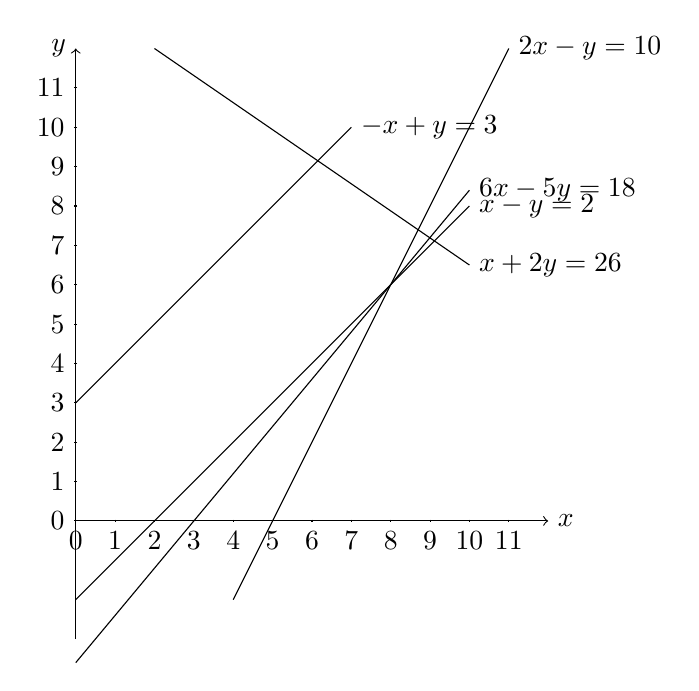
\begin{tikzpicture}[scale=0.5]
	\draw[->] (0,0) -- (12,0) node[below,right] {$x$};
	\draw[->] (0,-3) -- (0,12) node[above,left] {$y$};
	\draw (2,12) -- (10,6.5) node[above,right] {$x + 2y = 26$};
	\draw (0,3) -- (7,10) node[above,right] {$-x + y = 3$};
	\draw (0,-2) -- (10,8) node[above,right] {$x - y = 2$};
	\draw (4,-2) -- (11,12) node[above,right] {$2x - y = 10$};
	\draw (0,-3.6) -- (10,8.4) node[above,right] {$6x-5y = 18$};
	
	\foreach \x in {0,1,2,3,4,5,6,7,8,9,10,11}
	\draw (\x,1pt) -- (\x,-1pt) node[anchor=north] {$\x$};
	\foreach \y in {0,1,2,3,4,5,6,7,8,9,10,11}
	\draw (1pt,\y) -- (-1pt,\y) node[anchor=east] {$\y$};
	
	\end{tikzpicture}
\end{center}

\end{frame}

\end{document}
